134. \begin{figure}[ht!]
\center{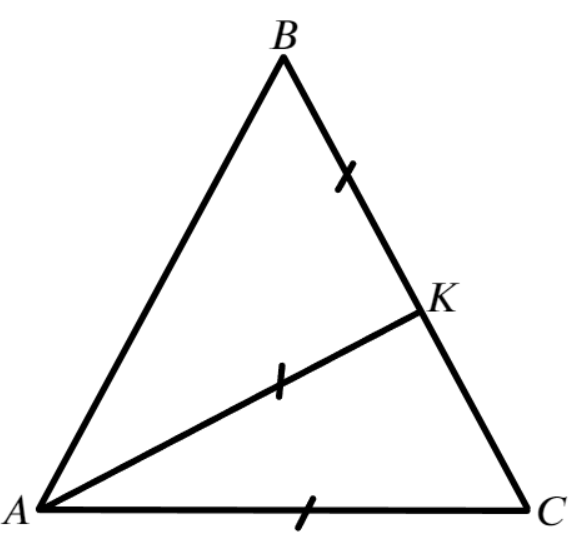
\includegraphics[scale=0.35]{g7-134.png}}
\end{figure}\\
Пусть $CA=AK=KB=x,$ а $KC=y,$ тогда $AB=CB=x+y$ и имеет место система уравнений $\begin{cases} 2x+y=4,\\ 3x+y=5.\end{cases}$ откуда $x=1,\ y=2.$ Но тогда в треугольнике $AKC$ получаем $AK+AC=1+1=2=CK,$ что невозможно по неравенству треугольника. Значит, такого треугольника не существует.
ewpage
oindent
